\begin{enumerate}[label=\thesubsection.\arabic*,ref=\thesubsection.\theenumi]
  \item Find the equation of the circle passing through the points $(4,1)$ and $(6,5)$ and whose centre is on the line $ 4x+y=16. $
\label{chapters/11/11/1/10}
\\
\solution
\iffalse

\documentclass[12pt]{article}
\usepackage{graphicx}
\usepackage{amsmath}
\usepackage{mathtools}
\usepackage{gensymb}

\newcommand{\mydet}[1]{\ensuremath{\begin{vmatrix}#1\end{vmatrix}}}
\providecommand{\brak}[1]{\ensuremath{\left(#1\right)}}
\providecommand{\norm}[1]{\left\lVert#1\right\rVert}
\newcommand{\solution}{\noindent \textbf{Solution: }}
\newcommand{\myvec}[1]{\ensuremath{\begin{pmatrix}#1\end{pmatrix}}}
\let\vec\mathbf

\begin{document}
\begin{center}
\textbf\large{CHAPTER-11 \\ CIRCLES}

\end{center}
\section*{Excercise 11.1}

Q10.Find the equation of the circle passing through the points $\brak{4,1} \text{ and } \brak{6,5}$ and whose centre is on the line $4x + y = 16$.

\solution
\fi
The equation of the circle is given by
\begin{align}
	\label{eq:chapters/11/11/1/10circEq1}
	\norm{\vec{x}}^2 + 2\vec{x}^\top \vec{u} + f = 0
\end{align}
where
\begin{align}
	\vec{u} &= -\vec{c}\\
	      f &= \norm{\vec{c}} - r^2
\end{align}
Given points are
\begin{align}
	\label{eq:chapters/11/11/1/10circPoints}
	\vec{x}_{1} = \myvec{4\\1} , \vec{x}_{2} = \myvec{6\\5}
\end{align}
And the line passing through the centre
\begin{align}
	\label{eq:chapters/11/11/1/10line1}
	\myvec{4 & 1}\vec{x} = 16
\end{align}
Substituting points from \eqref{eq:chapters/11/11/1/10circPoints} into \eqref{eq:chapters/11/11/1/10circEq1}
\begin{align}
	\brak{4^2 + 1^2}+2\myvec{4 & 1}\vec{u}+f&=0\\
	\label{eq:chapters/11/11/1/10eq1}	
	\implies 2\myvec{4 & 1}\vec{u}+f&=-17\\
	\brak{6^2 + 5^2}+2\myvec{6 & 5}\vec{u}+f&=0\\
	\label{eq:chapters/11/11/1/10eq2}
	\implies 2\myvec{6 & 5}\vec{u}+f&=-61
\end{align}
And since \eqref{eq:chapters/11/11/1/10line1} passes through the centre
\begin{align}
	-\vec{n}^\top \vec{u} &= c\\
	\label{eq:chapters/11/11/1/10eq3}
	-\myvec{4 & 1}\vec{u} &= 16
\end{align}
Representing \eqref{eq:chapters/11/11/1/10eq1},\eqref{eq:chapters/11/11/1/10eq2} and \eqref{eq:chapters/11/11/1/10eq3} in matrix form
\begin{align}
	\myvec{-4 & -1 & 0\\
	       12 & 10 & 1\\
	        8 &  2 & 1}
	\myvec{\vec{u}\\f} = 
	\myvec{16 \\ -61 \\ -17}
\end{align}
The augmented matrix is expressed as
\begin{align}
	\myvec{-4 & -1 & 0 & \vrule & 16\\
	       12 & 10 & 1 & \vrule & -61\\
	        8 &  2 & 1 & \vrule & -17}
\end{align}
Performing a sequence of row operations to transform into an Echelon form
\begin{align}
	\xleftrightarrow[R_2\rightarrow R_2+3R_1]{{R_3\rightarrow R_3+2R_1}}
	\myvec{-4 & -1 & 0 & \vrule & 16\\
	        0 &  7 & 1 & \vrule & -13\\
	        0 &  0 & 1 & \vrule & 15}\\
	\xleftrightarrow[]{{R_2\rightarrow R_2-R_3}}
	\myvec{-4 & -1 & 0 & \vrule & 16\\
	        0 &  7 & 0 & \vrule & -28\\
	        0 &  0 & 1 & \vrule & 15}\\
	\xleftrightarrow[]{{R_2\rightarrow \frac{R_2}{7},R_1\rightarrow \frac{-R_1}{4}}}
	\myvec{ 1 & \frac{1}{4} & 0 & \vrule & -4\\
	        0 &  1 & 0 & \vrule & -4\\
	        0 &  0 & 1 & \vrule & 15}\\
	\label{eq:chapters/11/11/1/10solution}	
	\xleftrightarrow[]{{R_1\rightarrow R_1-\frac{1}{4}R_2}}
	\myvec{ 1 &  0 & 0 & \vrule & -3\\
	        0 &  1 & 0 & \vrule & -4\\
	        0 &  0 & 1 & \vrule & 15}
\end{align}
So, from \eqref{eq:chapters/11/11/1/10solution}
\begin{align}
	\vec{u} &= \myvec{-3\\-4}\\
	f &= 15 
\end{align}
Since $\vec{u} = -\vec{c}$
\begin{align}
	\vec{c} &= \myvec{3\\4}\\
	r^2 &= \brak{3^2+4^2} - 15\\
	r &= \sqrt{10}
\end{align}
Hence, the equation of circle is
\begin{align}
	\norm{\vec{x}}^2 +2\vec{u}^\top \vec{x}+15 = 0\\
	\text{ where } \vec{u} = \myvec{-3\\-4}
\end{align}
The circle is plotted in Fig. \ref{fig:chapters/11/11/1/10Fig1}.
\begin{figure}[!h]
	\begin{center} 
	    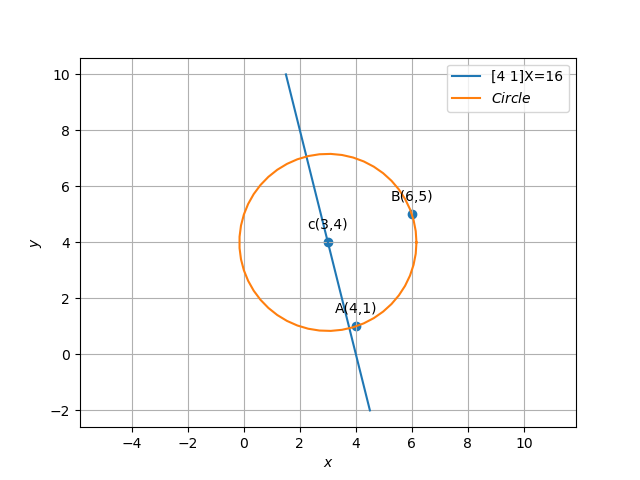
\includegraphics[width=\columnwidth]{chapters/11/11/1/10/figs/circ2}
	\end{center}
\caption{}
\label{fig:chapters/11/11/1/10Fig1}
\end{figure}






  \item Find the equation of the circle passing through the points $\vec{x}_1(2,3)$ and $\vec{x}_2(-1,1)$ and whose centre is on the line $x-3y-11=0$.
\label{chapters/11/11/1/11}
\\
\solution 
Substituting numerical values in 
	\eqref{eq:chapters/11/11/1/mat},
\begin{align}
	\label{eq:vertex_system}
	\myvec{4&6&1\\-2& 2&1\\-1& 3&0}\myvec{\vec{u}\\f} = \myvec{-13\\-2 \\11}
\end{align}
yielding
\begin{align}
	\vec{u}=\frac{1}{2}\myvec{-7 \\5},\
f=-14.
\end{align}
See Fig. 
	\begin{figure}[!ht]
		\centering
 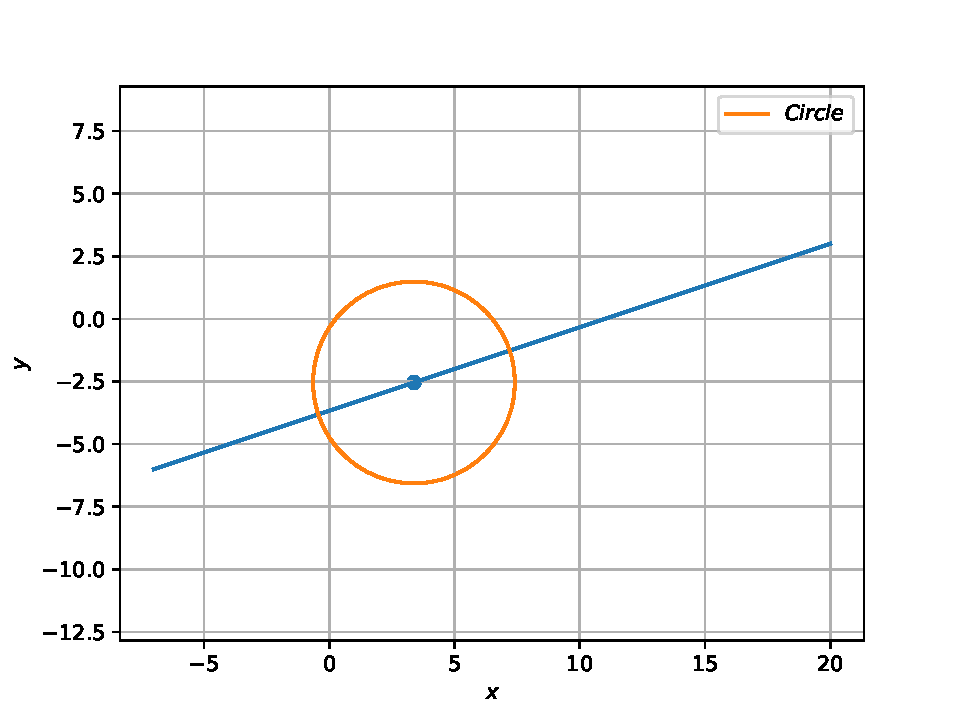
\includegraphics[width=\columnwidth]{chapters/11/11/1/11/figs/fig.pdf}
		\caption{}
		\label{fig:11/11/1/11}
  	\end{figure}

  \item Find the equation of the circle with radius 5 whose centre lies on $x$-axis and passes through the point $(2,3)$.
\label{chapters/11/11/1/12}
\\
\solution 
See 
		\figref{fig:11/11/1/12}.
	\begin{figure}[!ht]
		\centering
 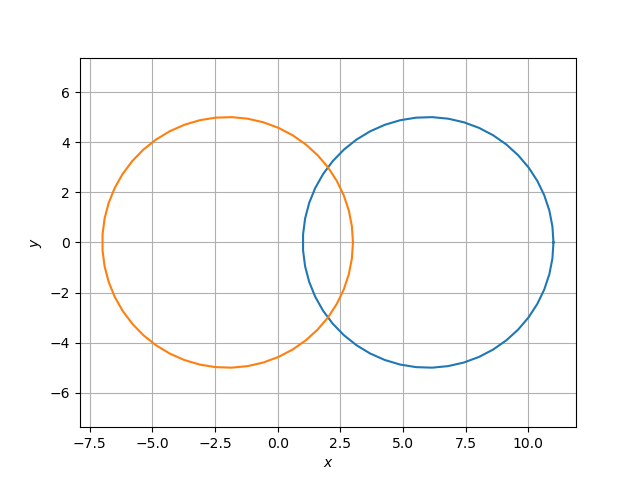
\includegraphics[width=\columnwidth]{chapters/11/11/1/12/figs/conic.png}
		\caption{}
		\label{fig:11/11/1/12}
  	\end{figure}
From the given information, the following equations can be formulated
using 
	\eqref{eq:circ-eq}.
\begin{align}
		\label{eq:11/11/1/12/1}
	\norm{\vec{P}}^2 + 2 \vec{u}^{\top}\vec{P} + f &= 0
	\\
		\label{eq:11/11/1/12/2}
	\vec{u} &= k\vec{e}_1
	\\
		\label{eq:11/11/1/12/3}
	\norm{\vec{u}}^2 - f &= r^2
\end{align}
where 
\begin{align}
	\vec{P} = \myvec{2\\3} \text{ and } r = 5
\end{align}
From 
		\eqref{eq:11/11/1/12/1}
		and 
		\eqref{eq:11/11/1/12/3},
\begin{align}
	\norm{\vec{P}}^2 + 2 \vec{u}^{\top}\vec{P} + \norm{\vec{u}}^2 &= r^2
\end{align}
Substituting from 
		\eqref{eq:11/11/1/12/2} in the above, 
\begin{align}
	k^2  + 2k \vec{e}_1^{\top}\vec{P} + \norm{\vec{P}}^2- r^2 = 0
\end{align}
resulting in 
\begin{align}
	k =  - \vec{e}_1^{\top}\vec{P} \pm \sqrt{\brak{{ \vec{e}_1^{\top}\vec{P}  }}^2 + r^2 - \norm{\vec{P}}^2 } 
\end{align}
Substituting numerical values, 
\begin{align}
	k = 2, -6
\end{align}
resulting in circles with centre
\begin{align}
	-\vec{u} = \myvec{-2 \\ 0} \text{ or } \myvec{6 \\ 0}.
\end{align}
This is verified in Fig. 
		\eqref{fig:11/11/1/12}.

  \item Find the equation of a circle with centre $(2,2)$ and passing through the point $(4,5)$.
\label{chapters/11/11/1/14}
\\
\solution
From the given information
\begin{align}
	\vec{u} = -\myvec{2\\2}, \, \vec{A} &= \myvec{4\\5}\\
\implies	\norm{\vec{A}}^2+2\vec{u}^\top\vec{A}+f &= 0\\
\implies	f = -\norm{\vec{A}}^2 - 2\vec{u}^\top\vec{A}
	&= -5
\end{align}
Hence the equation of circle is 
\begin{align}
	\norm{\vec{x}}^2+2\myvec{-2&-2}\vec{x}-5 = 0 	
\end{align}
See 
\figref{fig:chapters/11/11/1/14/1}.
\begin{figure}[H]
\centering
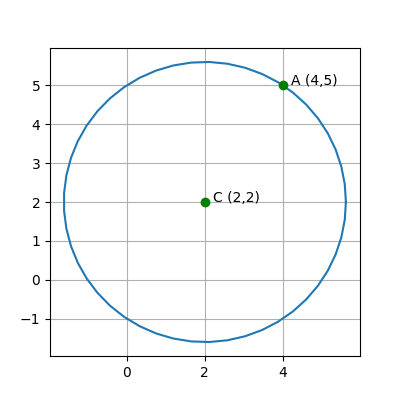
\includegraphics[width=0.75\columnwidth]{chapters/11/11/1/14/figs/fig.png}
\caption{}
\label{fig:chapters/11/11/1/14/1}
\end{figure}







  \item Does the point $(-2.5,3.5)$ lie inside, outside or on the circle $x^{2}+y^{2}=25?$
\\
\solution
See 
\tabref{tab:chapters/11/11/1/15/}.
\begin{table}[H]
\begin{center}
%%%%%%%%%%%%%%%%%%%%%%%%%%%%%%%%%%%%%%%%%%%%%%%%%%%%%%%%%%%%%%%%%%%%%%
%%                                                                  %%
%%  This is a LaTeX2e table fragment exported from Gnumeric.        %%
%%                                                                  %%
%%%%%%%%%%%%%%%%%%%%%%%%%%%%%%%%%%%%%%%%%%%%%%%%%%%%%%%%%%%%%%%%%%%%%%

\begin{tabular}[]{|c|c|}
\hline
Condition	&Inference		\\\hline
$\norm{\vec{x}-\vec{O}}^2<r^2$	&point lies inside the circle \\ \hline
$\norm{\vec{x}-\vec{O}}^2>r^2$	&point lies outside the circle \\ \hline
$\norm{\vec{x}-\vec{O}}^2=r^2$	&point lies on the circle \\ \hline	
\end{tabular}

\end{center}
\caption{}
\label{tab:chapters/11/11/1/15/}
\end{table}
The given circle equation can be expressed as
\begin{align}
	\norm{\vec{x}}^2= 25
\end{align}
Let,
\begin{align}
	\vec{P}=\myvec{-2.5\\3.5}
\end{align}
Since
\begin{align}
	\norm{\vec{P} - \vec{O}}^2 =
 18.5 < 25,
\end{align}
the point lies inside the given circle.
See 
    \figref{fig:chapters/11/11/1/15/}.
\begin{figure}[H]
  \centering
    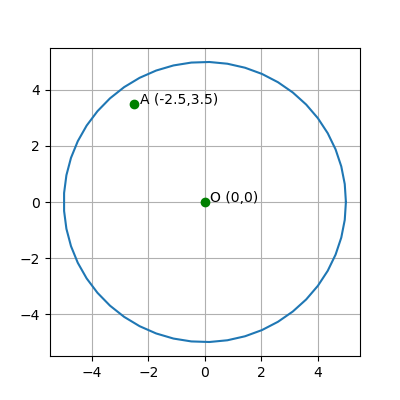
\includegraphics[width=0.75\columnwidth]{chapters/11/11/1/15/figs/Figure_1.png}
    \caption{}
    \label{fig:chapters/11/11/1/15/}
\end{figure}

\item Find the centre of a circle passing though the points $(6,-6), (3,-7)$ and $(3,3)$. \\ 
\label{chapters/10/7/4/3}
\solution 
\iffalse
\documentclass[12pt]{article}
\usepackage{graphicx}
\usepackage[none]{hyphenat}
\usepackage{graphicx}
\usepackage{listings}
\usepackage[english]{babel}
\usepackage{graphicx}
\usepackage{caption} 
\usepackage{booktabs}
\usepackage{array}
\usepackage{amssymb} % for \because
\usepackage{amsmath}   % for having text in math mode
\usepackage{extarrows} % for Row operations arrows
\usepackage{listings}
\lstset{
  frame=single,
  breaklines=true
}
\usepackage{hyperref}
  
%Following 2 lines were added to remove the blank page at the beginning
\usepackage{atbegshi}% http://ctan.org/pkg/atbegshi
\AtBeginDocument{\AtBeginShipoutNext{\AtBeginShipoutDiscard}}


%New macro definitions
\newcommand{\mydet}[1]{\ensuremath{\begin{vmatrix}#1\end{vmatrix}}}
\providecommand{\brak}[1]{\ensuremath{\left(#1\right)}}
\providecommand{\norm}[1]{\left\lVert#1\right\rVert}
\providecommand{\abs}[1]{\left\vert#1\right\vert}
\newcommand{\solution}{\noindent \textbf{Solution: }}
\newcommand{\myvec}[1]{\ensuremath{\begin{pmatrix}#1\end{pmatrix}}}
\let\vec\mathbf


\begin{document}

\begin{center}
\title{\textbf{Circles}}
\date{\vspace{-5ex}} %Not to print date automatically
\maketitle
\end{center}
\setcounter{page}{1}

\section{11$^{th}$ Maths - Chapter 10}
This is Problem-3 from Exercise 10.4
\begin{enumerate}
\fi
\solution 
The equation of the circle is given by 
\begin{align}
	\label{eq:10/7/4/3circEq1}
	\norm{\vec{x}}^2+2\vec{x}^\top\vec{u}+f = 0 
\end{align}
where
\begin{align}
	\vec{u} = -\vec{c} \text{ and } \\
        \label{eq:10/7/4/3fRelation}
	f = \norm{\vec{c}}^2 - r^2
\end{align}
Given points are 
\begin{align}
	\label{eq:10/7/4/3circPoints}
     \vec{x_1} = \myvec{6 \\ -6} , \vec{x_2} = \myvec{3 \\-7}, \vec{x_3}= \myvec{3 \\ 3}
\end{align}
Substituting points from \eqref{eq:10/7/4/3circPoints} into \eqref{eq:10/7/4/3circEq1}
\begin{align}
	\brak{6^2 + \brak{-6}^2}+2\myvec{6 & -6}\vec{u}+f = 0 \\ 
	\implies 2\myvec{6 & -6}\vec{u} + f = -72 \\ 
	\brak{3^2 + \brak{-7}^2}+2\myvec{3 & -7}\vec{u}+f = 0 \\ 
	\implies 2\myvec{3 & -7}\vec{u} + f = -58 \\
	\brak{3^2 + 3^2}+2\myvec{3 & 3}\vec{u}+f = 0 \\ 
	\implies 2\myvec{3 & 3}\vec{u} + f = -18 
\end{align}
Representing the above system of equations in matrix form
\begin{align}
 \myvec{6 & -14 & 1 \\
	12 & -12 & 1 \\
	6 & 6 & 1
	} \myvec {\vec{u} \\
	           f 
		}  = \myvec{-58 \\ -72 \\ -18 }
\end{align}

The augmented matrix is expressed as
\begin{align}
	\myvec{6 & -14 & 1 & \vrule & -58 \\ 
	      12 & -12 & 1 & \vrule & -72 \\
	       6 &  6  & 1 & \vrule & -18 
	     }  
\end{align}
Performing sequence of row operations to transform into an Echelon form
\begin{align}
	\xleftrightarrow[]{{R_2\rightarrow R_2-2R_1}}  
	\myvec{6 & -14 & 1 & \vrule & -58 \\ 
	       0 &  16 & -1 & \vrule & 44 \\
	       6 &  6  & 1 & \vrule & -18 
	     }  \\ 
	\xleftrightarrow[]{{R_3\rightarrow R_3-R_1}}  
	\myvec{6 & -14 & 1 & \vrule & -58 \\ 
	       0 &  16 & -1 & \vrule & 44 \\
	       0 &  20  & 0 & \vrule & 40 
	     }  
\end{align}
\begin{align}
	\xleftrightarrow[]{{R_3\rightarrow R_3-\frac{20}{16}R_2}}  
	\myvec{6 & -14 & 1 & \vrule & -58 \\ 
	       0 &  16 & -1 & \vrule & 44 \\
	       0 &  0  &  \frac{20}{16} & \vrule & -15 
	     }  \\ 
	\xleftrightarrow[R_2\rightarrow \frac{1}{16}R_2 \text{,} R_3\rightarrow \frac{16}{20}R_3]{{R_1\rightarrow \frac{1}{6}R_1}}  
	\myvec{1 & -\frac{14}{6} & \frac{1}{6} & \vrule & -\frac{58}{6} \\ 
	       0 &  1 & -\frac{1}{16} & \vrule & \frac{44}{16} \\
	       0 &  0  &  1  & \vrule & -12 
	     }   
\end{align}
\begin{align}
	\xleftrightarrow[R_2\rightarrow R_2+\frac{1}{16}R_3]{{R_1\rightarrow R_1-\frac{1}{6}R_3}}  
	\myvec{1 & -\frac{14}{6} & 0 & \vrule & -\frac{46}{6} \\ 
	       0 &  1 & 0 & \vrule & 2 \\
	       0 &  0  &  1  & \vrule & -12 
	     }  \\ 
	\label{eq:10/7/4/3Solution}
	\xleftrightarrow[]{{R_1\rightarrow R_1+\frac{14}{6}R_2}}  
	\myvec{1 &  0 & 0 & \vrule & -3\\ 
	       0 &  1 & 0 & \vrule & 2 \\
	       0 &  0 & 1 & \vrule & -12 
	     }  
\end{align}
So, from  \eqref{eq:10/7/4/3Solution} 
\begin{align}
	\vec{u} = \myvec{-3 \\ 2} \\ 
	f = -12 
\end{align}
Since $\vec{u} = -\vec{c}$ , 
\begin{align}
	\vec{c} &= \myvec{ 3 \\ -2} \\
	\eqref{eq:10/7/4/3fRelation} \implies r^2 &= \brak{3^2 + \brak{-2}^2} + 12 \\
	 r &= 5
\end{align}
Therefore, the equation of the circle is 
\begin{align}
	\norm{\vec{x}-\myvec{3 \\ -2}}  = 5 
\end{align}
The relevant diagram is shown in Figure \ref{fig:10/7/4/3Fig1}
\begin{figure}[!h]
	\begin{center}
		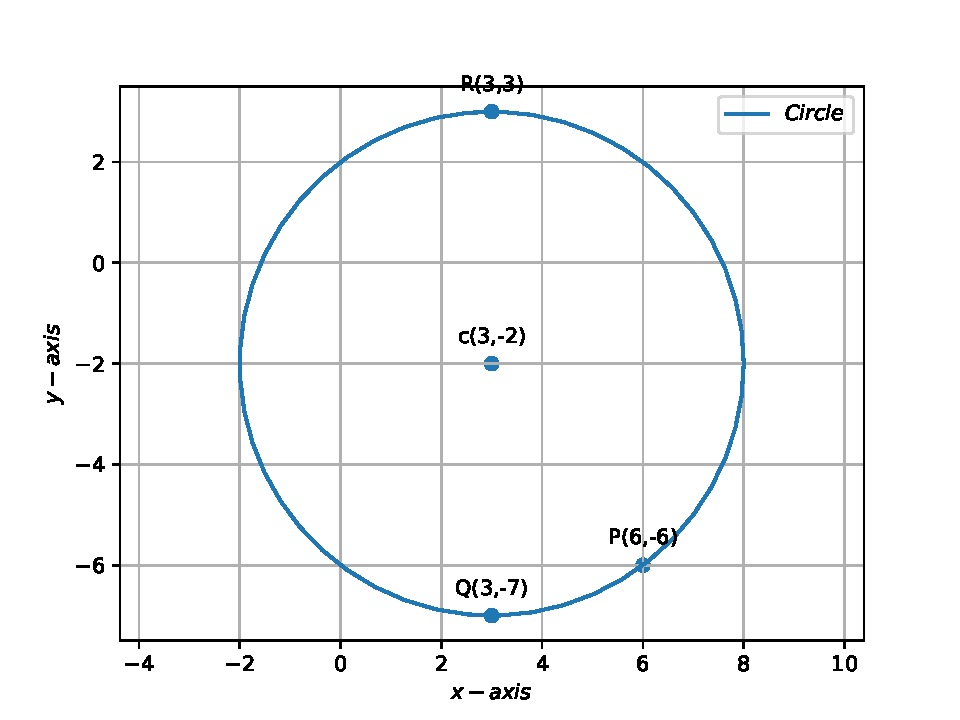
\includegraphics[width=\columnwidth]{chapters/10/7/4/3/figs/problem3.pdf}
	\end{center}
\caption{}
\label{fig:10/7/4/3Fig1}
\end{figure}

  \item Find the equation of the circle passing through $(0,0)$ and making intercepts $a$ and $b$ on the coordinate axes.
\end{enumerate}
In each of the following exercises, find the equation of the circle with the following parameters
\begin{enumerate}[label=\thesubsection.\arabic*,ref=\thesubsection.\theenumi,resume*]
 \item centre $(0,2)$ and radius $2$
	 \\
		\solution
\label{chapters/11/11/1/1}
Substituting numerical values in 
	\eqref{eq:circ-cr},
\begin{align}
	\vec{u} = \myvec{0\\-2},
	f 
	  = 0
\end{align}
Thus, the equation of circle is obtained as
\begin{align}
	\norm{\vec{x}}^2 - 2\myvec{0 & 2}\vec{x} = 0
\end{align}
\iffalse
See \figref{fig:11/11/1/1/Fig1}.
\begin{figure}[H]
	\begin{center} 
	    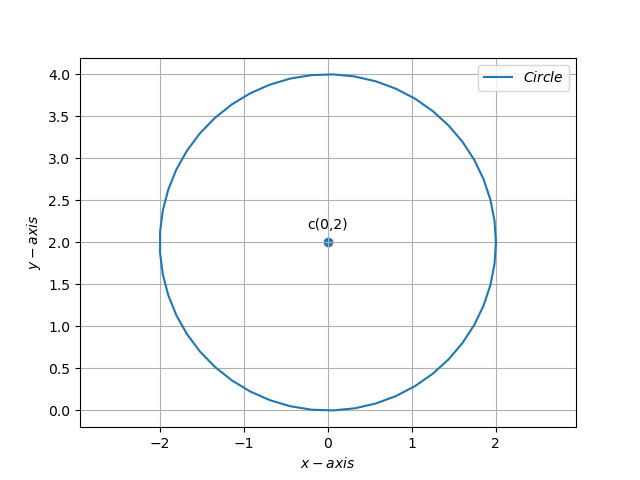
\includegraphics[width=0.75\columnwidth]{chapters/11/11/1/1/figs/circ1}
	\end{center}
\caption{}
\label{fig:11/11/1/1/Fig1}
\end{figure}
\fi

%
  \item centre $(-2,3)$ and radius 4
	 \\
		\solution
\label{chapters/11/11/1/2}
Given
\begin{align}
	\vec{u} = -\myvec{-2\\3},  r = 4.
\end{align}
Substituting in 
	\eqref{eq:circ-cr},
\begin{align}
	f = -3
\end{align}
The equation of the circle is then obtained as
\begin{align}
	\norm{\vec{x}}^2 + 2\myvec{2&-3}\vec{x} -3=0     		       
\end{align}	
See  
\figref{fig:chapters/11/11/1/2/Fig1}.
\begin{figure}[H]
	\begin{center} 
	    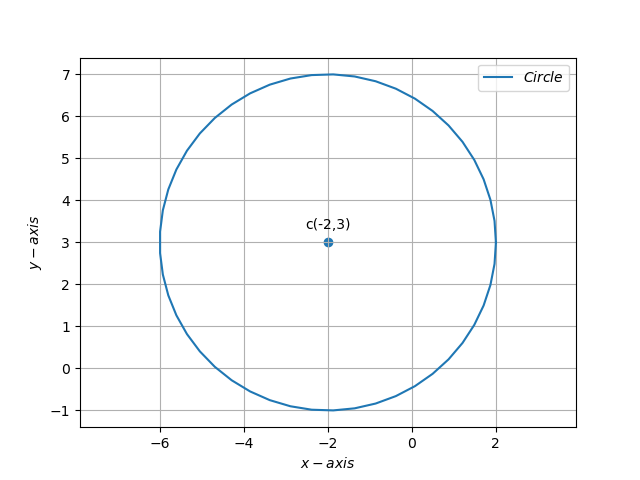
\includegraphics[width=0.75\columnwidth]{chapters/11/11/1/2/figs/circle.png}
	\end{center}
\caption{}
\label{fig:chapters/11/11/1/2/Fig1}
\end{figure}



  \item centre $\left(\frac{1}{2}, \frac{1}{4}\right)$ and radius $\frac{1}{12}$
\label{chapters/11/11/1/3}
	 \\
		\solution
Substituting numerical values
	in \eqref{eq:circ-cr},
\begin{align}
	f
	=\frac{11}{36}
\end{align}
	Thus, the equation of the circle is
\begin{align}
	\norm{\vec{x}}^2 + \myvec{-1 & -\frac{1}{2}}\vec{x}+\frac{11}{36}=0
\end{align}
\iffalse
See \figref{fig:chapters/11/11/1/3/Fig1}.
\begin{figure}[H]
\begin{center}
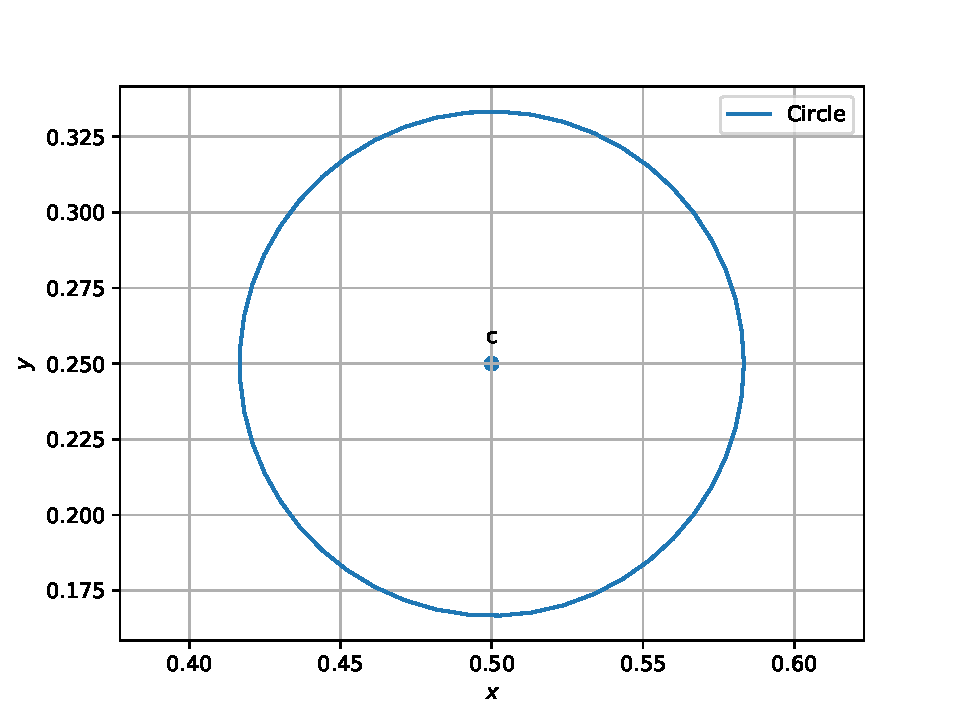
\includegraphics[width=0.75\columnwidth]{chapters/11/11/1/3/figs/fig.pdf}
\end{center}
\caption{}
\label{fig:chapters/11/11/1/3/Fig1}
\end{figure}
\fi

  \item centre $(1,1)$ and radius $\sqrt{2}$
	 \\
		\solution
Substituting
\begin{align}
	 r = \sqrt{2},\
	\vec{u}
	 = \myvec{-1\\-1}
\end{align}
in 
	\eqref{eq:circ-cr},
\begin{align}
	f 
	  =0	
\end{align}
Thus, the equation of the circle is 
\begin{align}
	\norm{\vec{x}}^2 -2\myvec{1&1}\vec{x} = 0       		       
\end{align}	
See 
\figref{fig:chapters/11/11/1/4/Fig1}.
\begin{figure}[!ht]
	\begin{center} 
	  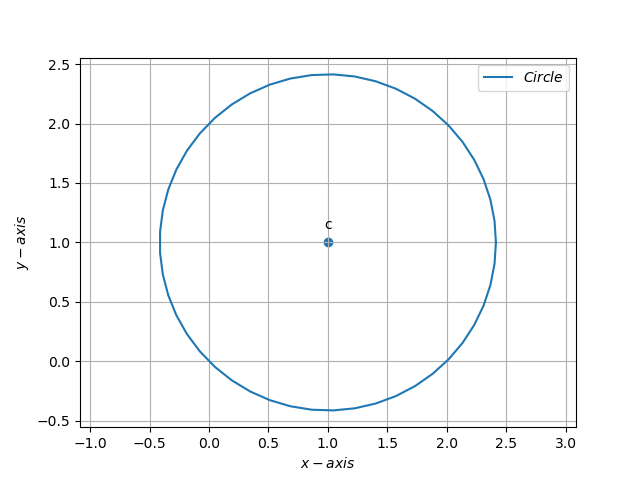
\includegraphics[width=\columnwidth]{chapters/11/11/1/4/figs/circ.png}
	\end{center}
\caption{}
\label{fig:chapters/11/11/1/4/Fig1}
\end{figure}


  \item centre $(-a,-b)$ and radius $\sqrt{a^{2}-b^{2}}$.
	 \\
		\solution
\label{chapters/11/11/1/5}
%	From \eqref{eq:circ-cr},
\begin{align}
	\vec{u} &= \myvec{a\\b},\,
	f  
	  =2b^2
\end{align}
Thus, the equation of circle is 
\begin{align}
	\norm{\vec{x}}^2 +2 \myvec{a&b}\vec{x}+2b^2 &= 0       		       
\end{align}	

\end{enumerate}

In each of the following exercises,  find the centre and radius of the circles.
\begin{enumerate}[label=\thesection.\arabic*,ref=\thesection.\theenumi,resume*]
\item  $x^2+y^2 +10x -6y -2=0$. 
	 \\
		\solution
\label{chapters/11/11/1/6}
%\iffalse
\documentclass[12pt]{article}
\usepackage{graphicx}
%\documentclass[journal,12pt,twocolumn]{IEEEtran}
\usepackage[none]{hyphenat}
\usepackage{graphicx}
\usepackage{listings}
\usepackage[english]{babel}
\usepackage{graphicx}
\usepackage{caption} 
\usepackage{hyperref}
\usepackage{booktabs}
\def\inputGnumericTable{}
\usepackage{color}                                            %%
    \usepackage{array}                                            %%
    \usepackage{longtable}                                        %%
    \usepackage{calc}                                             %%
    \usepackage{multirow}                                         %%
    \usepackage{hhline}                                           %%
    \usepackage{ifthen}
\usepackage{array}
\usepackage{amsmath}   % for having text in math mode
\usepackage{listings}
\lstset{
language=tex,
frame=single, 
breaklines=true
}
  
%Following 2 lines were added to remove the blank page at the beginning
\usepackage{atbegshi}% http://ctan.org/pkg/atbegshi
\AtBeginDocument{\AtBeginShipoutNext{\AtBeginShipoutDiscard}}
%
%New macro definitions
\newcommand{\mydet}[1]{\ensuremath{\begin{vmatrix}#1\end{vmatrix}}}
\providecommand{\brak}[1]{\ensuremath{\left(#1\right)}}
\providecommand{\norm}[1]{\left\lVert#1\right\rVert}
\newcommand{\solution}{\noindent \textbf{Solution: }}
\newcommand{\myvec}[1]{\ensuremath{\begin{pmatrix}#1\end{pmatrix}}}
\let\vec\mathbf
\begin{document}
\begin{center}
\title{\textbf{Circles}}
\date{\vspace{-5ex}} %Not to print date automatically
\maketitle
\end{center}
\setcounter{page}{1}
\section{11$^{th}$ Maths - Chapter 11}
\textbf{This is Problem-6 from Exercise 11.1 }

Q2. Find the centre and radius of the given circle $(\vec{x} + 5)^2 + (\vec{y} – 3)^2 = 36.$

\solution
\\
Given circle equation is
\begin{align}
	(\vec{x} + 5)^2 + (\vec{y} – 3)^2 = 36 \label{1}
\end{align}
The general equation of  the circle is 
\begin{align}
	\norm{\vec{x}}^{2} + 2\vec{u}^{\top}\vec{x} + f = 0
\end{align}
Where,
\begin{align}
	\vec{u} &= -\vec{c} \text{ and } f = \norm{\vec{u}}^{2} - r^{2}\label{3}
\end{align}
by expanding \eqref{1}
\begin{align}
	\vec{x}^2+10\vec{x}+25+\vec{y}^2-6\vec{y}+9-36&=0\\
	\norm{\vec{x}}^2+2\myvec{5 & -3}\vec{x}-2&=0\label{6}
\end{align}	
by comparing \eqref{3} to \eqref{6} we get
\fi
The circle parameters are
\begin{align}
 \vec{u}=\myvec{5\\ -3},\,
 f&=-2\\
\implies \vec{c}=\myvec{-5 \\ 3},\,
	r=\sqrt{\norm{\vec{u}}^2-f}
&= 6
\end{align}
See Fig. 
\ref{fig:chapters/11/11/1/6/Fig1}.
\begin{figure}[!h]
	\begin{center} 
	   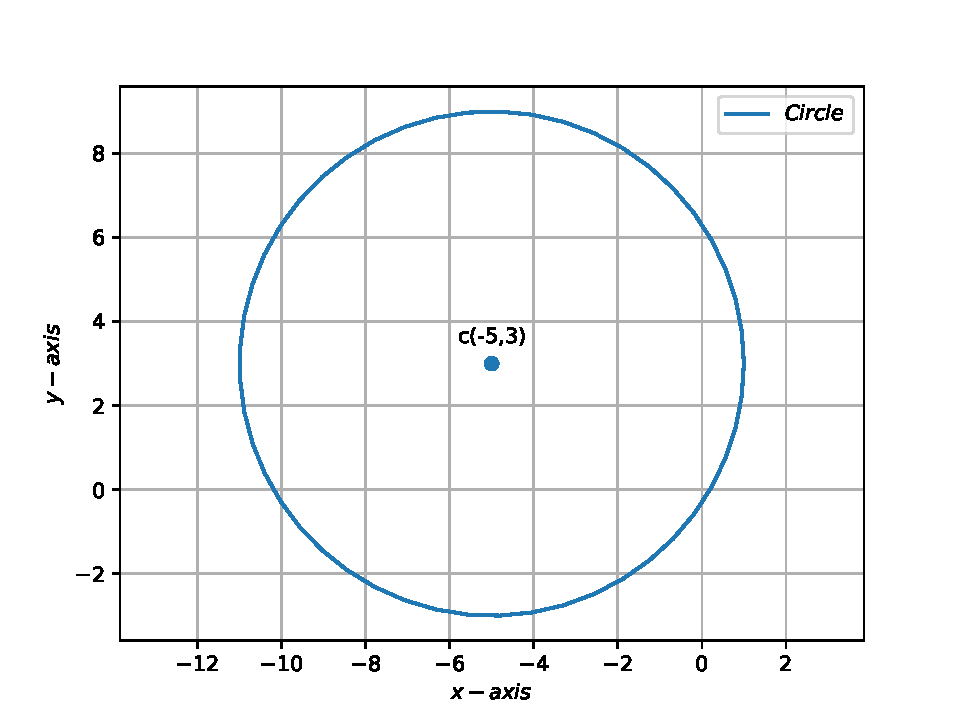
\includegraphics[width=\columnwidth]{chapters/11/11/1/6/figs/fig.pdf}
	\end{center}
\caption{}
\label{fig:chapters/11/11/1/6/Fig1}
\end{figure}


\item  $x^{2}+y^{2}-4 x-8 y-45=0$
	 \\
		\solution
\label{chapters/11/11/1/7}
%The given circle can be expressed as
\begin{align}
    \label{eq:chapters/11/11/1/7/given} 
    \norm{\vec{x}}^2  + 2\myvec{-2 & -4}\vec{x} - 45 = 0
\end{align}
where
\begin{align}	
	\vec{u} &= \myvec{-2\\-4},\, f = -45 \\
	\implies \vec{c} &= \myvec{2\\4},\,
	r = \sqrt{65}.	
\end{align}
\iffalse
See Fig. 
    \ref{fig:chapters/11/11/1/7/cicle}.
\begin{figure}[H]
    \centering
    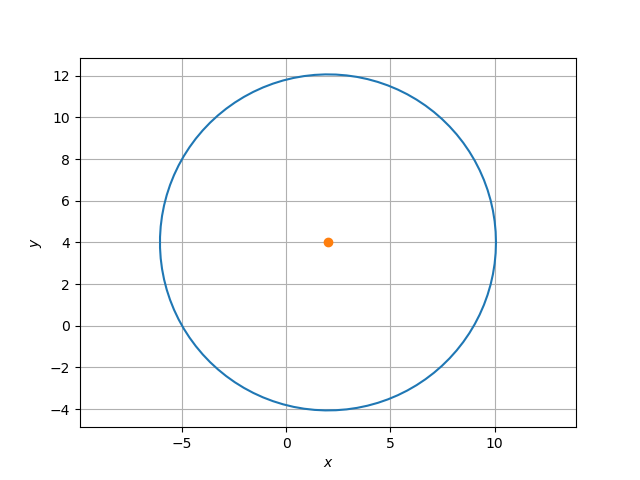
\includegraphics[width=0.75\columnwidth]{chapters/11/11/1/7/figs/circle.png}
    \caption{}
    \label{fig:chapters/11/11/1/7/cicle}
\end{figure}
\fi


\item  $x^{2}+y^{2}-8 x+10 y-12=0$ 
	 \\
		\solution
\label{chapters/11/11/1/8}
%From the given informtion,
\begin{align}
 \vec{u}=\myvec{-4\\5},\,
 f&=-12\\
\implies \vec{c}&=\myvec{4 \\ -5},\\
	r=\sqrt{\norm{\vec{u}}^2-f}
&=\sqrt{53}
\end{align}
See Fig. 
\ref{fig:chapters/11/11/1/8/Fig1}.
\begin{figure}[H]
	\begin{center} 
	   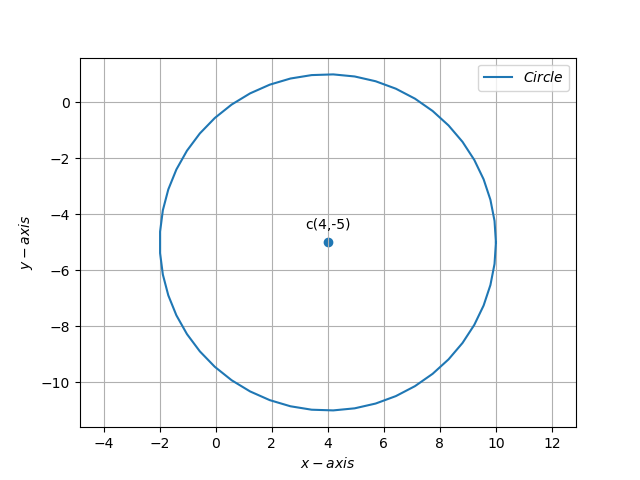
\includegraphics[width=0.75\columnwidth]{chapters/11/11/1/8/figs/11.1.8.png}
	\end{center}
\caption{}
\label{fig:chapters/11/11/1/8/Fig1}
\end{figure}

\item  $2 x^{2}+2 y^{2}-x=0$
	 \\
		\solution
\label{chapters/11/11/1/9}
%The given equation can be expressed as 
\begin{align}
\norm{\vec{x}}^2+2\myvec{\frac{-1}{4} & 0}\vec{x}&=0
\end{align}	
The centre of circle is then given by 
\begin{align}
	\vec{u} = -\vec{c} 
=\myvec{\frac{1}{4}\\0}
\end{align}
and the radius of circle is obtained as
\begin{align}
	r=\sqrt{\norm{\vec{u}}^2 -f}
=\frac{1}{4}
\end{align}
See 
  \figref{fig:chapters/11/11/1/9/Figure}.
\begin{figure}[H]
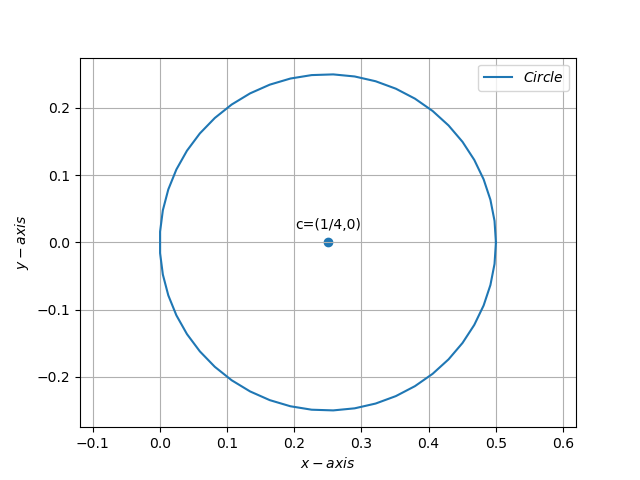
\includegraphics[width=0.75\columnwidth]{chapters/11/11/1/9/figs/fig.png}
\caption{}
  \label{fig:chapters/11/11/1/9/Figure}
\end{figure}

\item
%Find the equation of the circle with radius 5 whose centre lies on $x$-axis and passes through the point $\brak{2,3}$.

\textbf{Solution :}
\begin{table}[H]
    \centering
        \begin{tabular}{|c|c|c|}
    \hline
         \textbf{Input parameters}& \textbf{Description}&\textbf{Value} \\
         \hline
         $r$ & Radius&$5$ \\
        \hline
        $\vec{O}$ & Center&$x\vec{e_1}$ \\
        \hline
       $\vec{A}$&Point &$\myvec{2\\3}$ \\
       \hline
    \end{tabular}

        \caption{Table of input parameters}
    \label{tab:11.11.1.13}
\end{table}
The general formula of the circle is
\begin{align}
\norm{\vec{x}}^2 + 2\vec{u}^{\top}\vec{x}+f&=0\\
	where,   \vec{u}&=-x\vec{e_1}\\
	f&=\norm{\vec{O}}-r^2\\
f&=x-r^2\\
\norm{\vec{A}}^2 + 2\vec{u}^{\top}\vec{A}+f&=0\\
13-4x+x-r^2&=0\\
or,x&=-4\\
or,f&=-29
\end{align}
Therefore the equations of the circle are
\begin{align}
   \norm{\vec{x}}^2 - 2\myvec{-4&0}\vec{x}-29&=0\\
\end{align}    
\begin{figure}[H]
    \centering
	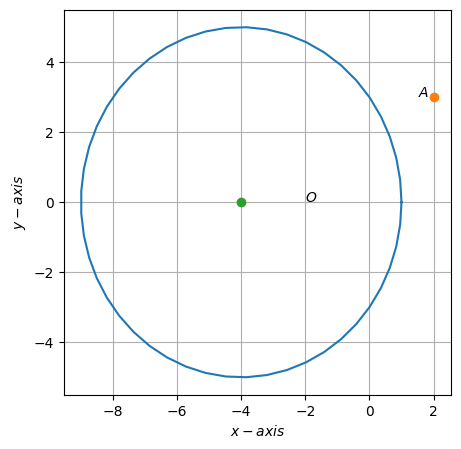
\includegraphics[width=\columnwidth]{chapters/11/11/1/13/fig/11.11.1.13.png}
    \caption{}
    \label{fig:11.11.1.13}
\end{figure}



\end{enumerate}
